\documentclass[exercice,a4]{thedocument}%
\usepackage{texmaths-tikz}%
\usepackage{tabularray}%
\usepackage{scratch3}%
\usepackage[np]{numprint}%
\startdatakeys
\source{24GENMATG11}
\BO{2026}
\cycle{4}
\competencesDuSocle{CA,RA}
\objectifsApprentissage{C4A1af,C4A1ee,C4A2ad,C4A2eb,C4A2ed,C4E1ad}
\motsCles{programme de calcul,expression littérale,développement,factorisation,équation,fonction,graphique}
\enddatakeys
\begin{document}%
On considère le programme de calcul suivant :

\begin{center}
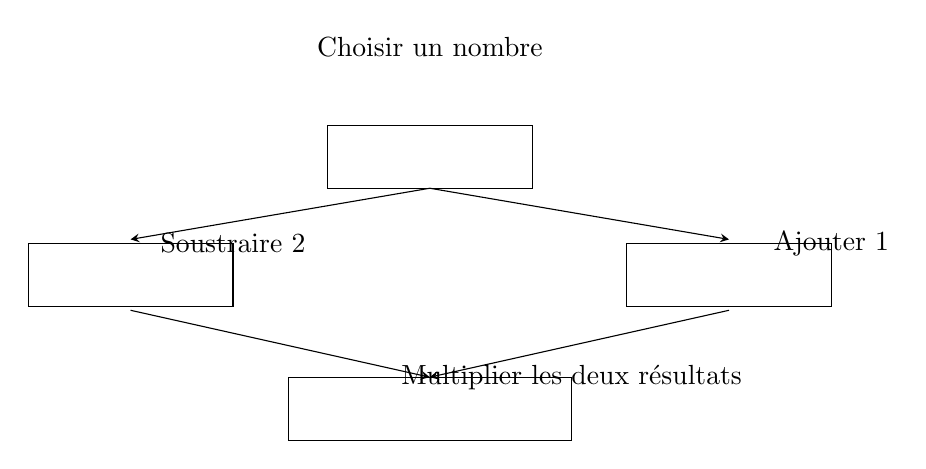
\begin{tikzpicture}[>=stealth]
    \node at(0,4.4){Choisir un nombre};
    \draw[shift={(0,3)}](-1.3,-.4)rectangle(1.3,.4);
    \draw[shift={(-3.8,1.5)}](-1.3,-.4)rectangle(1.3,.4)
        node{Soustraire 2};
    \draw[shift={(3.8,1.5)}](-1.3,-.4)rectangle(1.3,.4)
        node{Ajouter 1};
    \draw[shift={(0,-.2)}](-1.8,-.4)rectangle(1.8,.4)
        node{Multiplier les deux résultats};
    \draw[->](0,2.6)--(-3.8,1.95);
    \draw[->](0,2.6)--(3.8,1.95);
    \draw[->](-3.8,1.05)--(0,.2);
    \draw[->](3.8,1.05)--(0,.2);
\end{tikzpicture}
\end{center}

\textbf{Partie A}
\begin{enumerate}
    \item Justifier qu'en choisissant 5 comme nombre de départ, le résultat
    final est 18.
    \item Calculer le résultat lorsque le nombre de départ est
    $-\dfrac32$.
    \item Compléter les lignes 3, 4 et 5 du script correspondant au
    programme de calcul.
\end{enumerate}

\textbf{Partie B}

Soit $g$ définie par $g(x)=x^2-x-2$.
\begin{enumerate}
    \item Prouver que $(x-2)(x+1)=x^2-x-2$.
    \item
    \begin{enumerate}
        \item Résoudre $(x-2)(x+1)=0$.
        \item En déduire les antécédents de 0 par $g$.
    \end{enumerate}
    \item Parmi les graphiques proposés, choisir celui qui représente $g$.
    \item Quels nombres choisir au départ pour que le programme donne 0 ?
\end{enumerate}
\showthesource
\end{document}
